\documentclass[a4paper,12pt]{article}
\usepackage{fancyvrb}
\usepackage{algorithm}
\usepackage{algorithmic}
\usepackage{graphicx}
\usepackage{caption}
\usepackage{float}
% \usepackage[style=alphabetic]{biblatex}
\usepackage{color, amsmath, amssymb}


\begin{document}
\title{Enhancing Hi-C contact map resolution by neural networks}
\author{Minggu Wang \and Osamu Maruyama}
\maketitle

\section{Background}

\textcolor{red}{Wang-kun, please put important references here.}


\section{Methods}

A contact map usually formed as  an $n \times n$ matrix. The whole genome divided into n sized bins. Coordinate $(i,j)$ in contact map represents the number of interactions between bin i and bin j on the chromosome. Each contact map has a corresponding resolution, which indicates the range of each cell of the contact map.


Let $D$ be a set of paired ends reads of a Hi-C experiment. 
We generate low and high contact maps from $D$, 
denoted by $M_\ell$ and $M_h$ of size $S_\ell$ and $S_h$, respectively.  
Let $R = \frac{S_\ell}{S_h}$, \textit{i.e.}, 
the ratio of $S_\ell$ to $S_h$.  

Let $P$ be the number of overlapping pixels between adjacent sub-maps.
Let $K$ be the size of low-resolution sub-maps.

\begin{algorithm}[htbp]
\caption{Generating submatrices of $M_\ell$}
\begin{algorithmic}
% Divide matrices $M_\ell$ and $M_h$ \
    \FOR {$i = 1, 1 + K-P, 1+2\times(K-P)$, ..., $S_\ell-K+1$}
        \FOR {$j = 1, 1+K-P, 1+2\times(K-P)$, ..., $S_\ell-K+1$}
            \IF {$i+K > M_\ell$ \OR $j+K > M_\ell$} 
                \STATE break;
            \ELSE 
                \STATE extract $K \times K$ sub-maps whose left-top coordinate is $(i,j)$ from $M_\ell$;
            \ENDIF    
        \ENDFOR
    \ENDFOR
\end{algorithmic}
\end{algorithm}

\begin{algorithm}[htbp]
\caption{Generating submatrices of $M_h$}
\begin{algorithmic}
   \FOR {$i = 1, 1+(K-P) \times R, 1+2\times(K-P) \times R$, ..., $S_h-K+1$}
       \FOR {$j = 1, 1+(K-P) \times R, 1+2\times(K-P) \times R$, ..., $S_h-K+1$}
            \IF {$i+K \times R > M_h$ \OR $j+K \times R > M_h$}
                \STATE break; 
            \ELSE 
                \STATE extract $(K \times R) \times (K \times R)$sub-maps whose left-top coordinate is $(i,j)$ from $M_h$;
            \ENDIF
        \ENDFOR
    \ENDFOR    
\end{algorithmic}
\end{algorithm}

\begin{figure}[htbp]
\centering
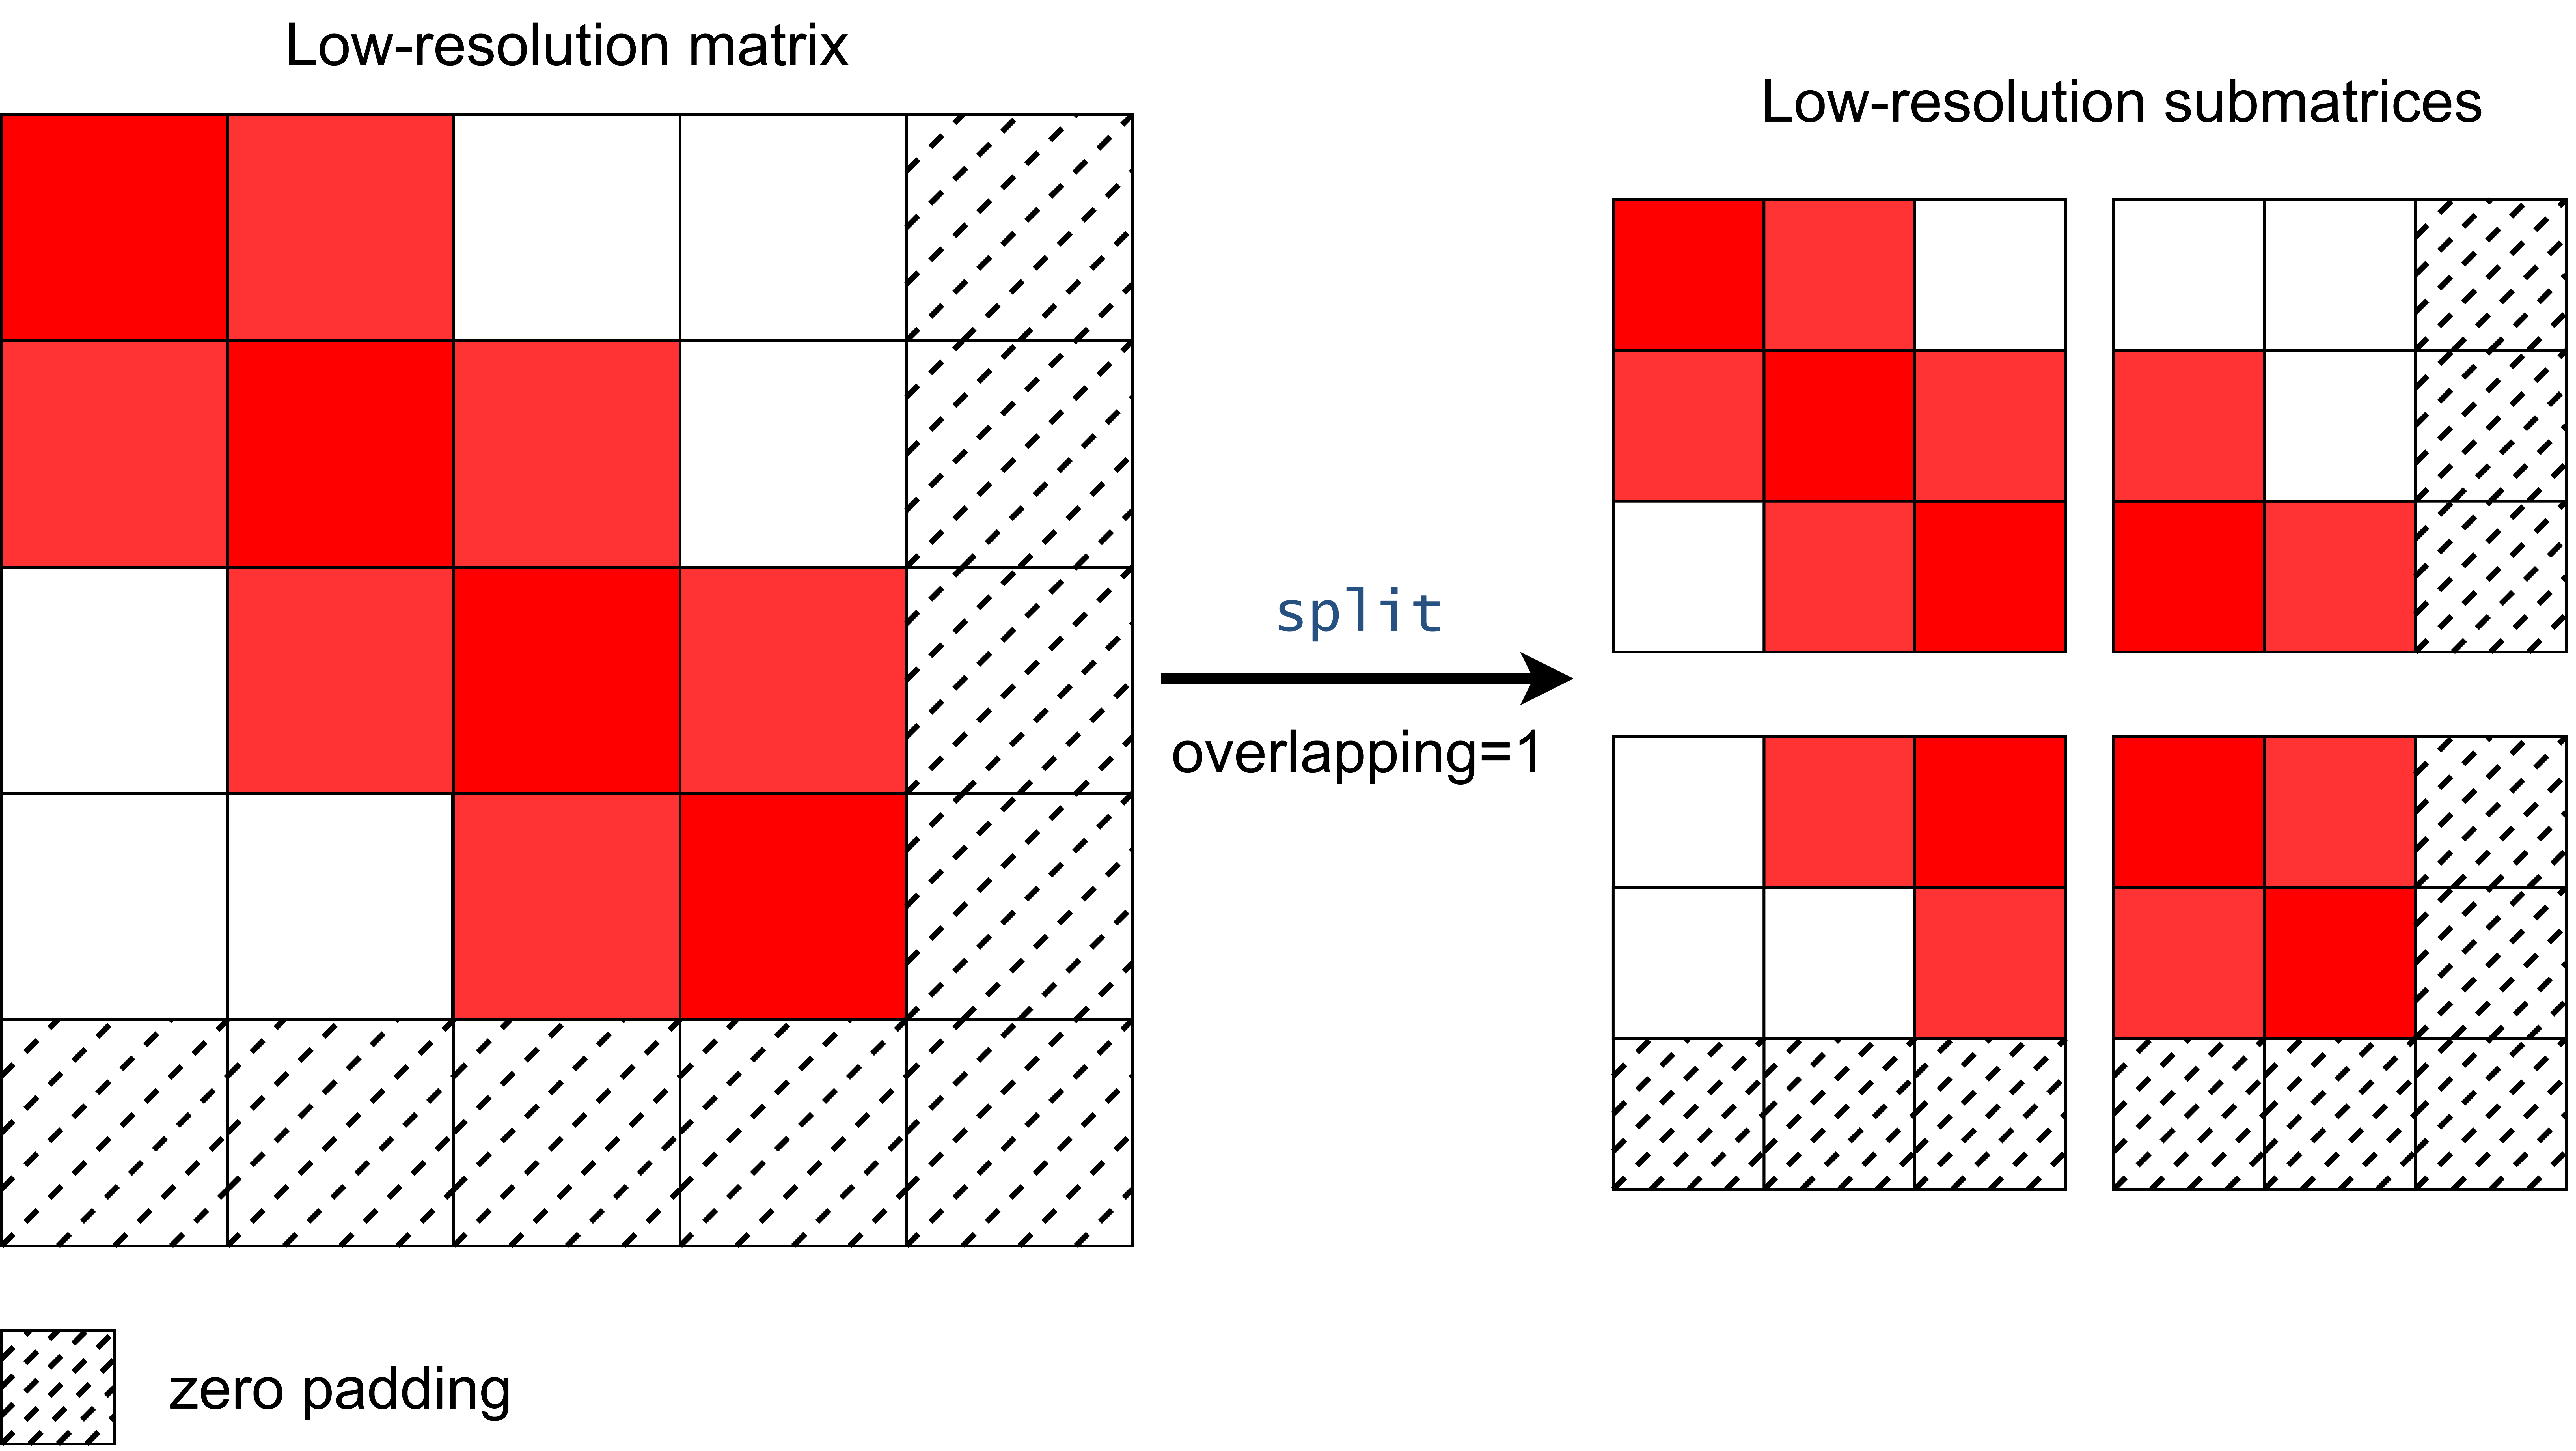
\includegraphics[scale=0.03]{figures/lowres_split.png}
\caption{Split low-resolution matrix to submatrices}
\label{low-res to submatrices}
\end{figure}

\begin{figure}[htbp]
\centering
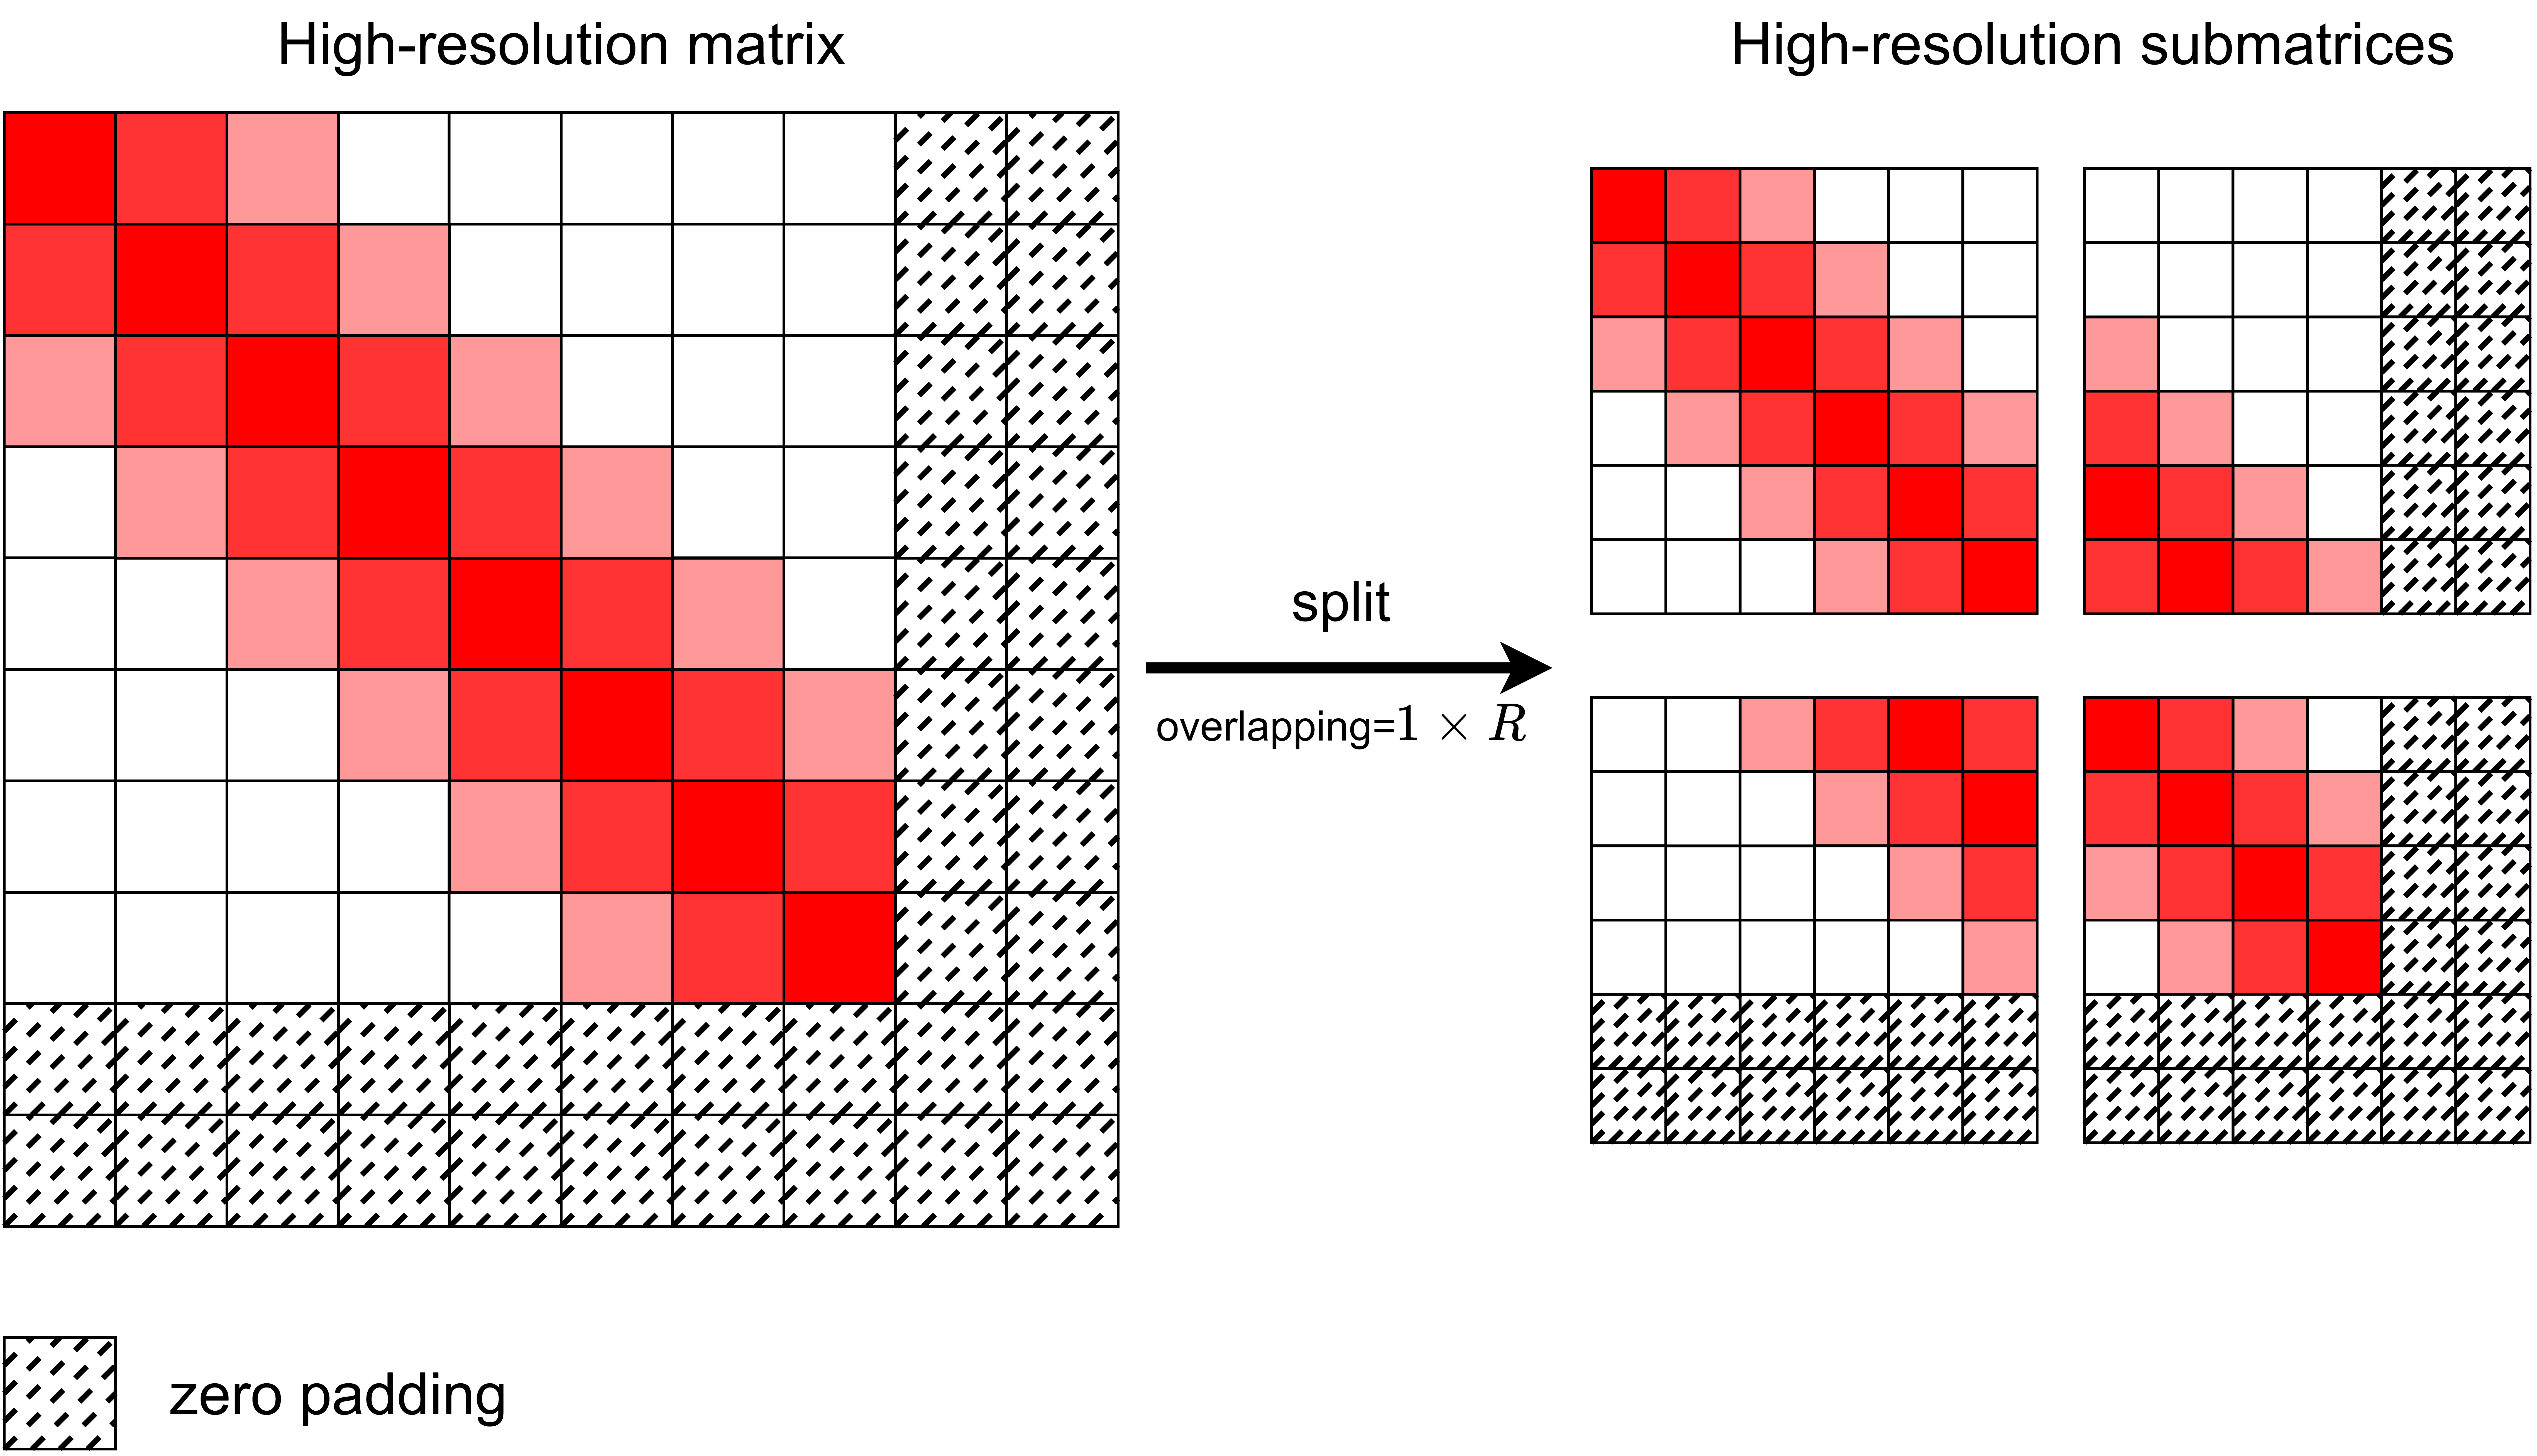
\includegraphics[scale=0.03]{figures/highres_split.png}
\caption{Split high-resolution matrix to submatrices}
\end{figure}
% training part: 


Let $C_\ell$ and $C_h$ be collections of the resulting low-resolution and high-resolution
sub-maps. Let $\hat{C_h}$ be the collection of the high-resolution sub-matrices generated by neural network. We train a neural network using $C_\ell$ and $C_h$. The mean square error(MSE) is used as 
loss function in the training process. 



\begin{center}
    $MSE[C_\ell, C_h] = \frac{1}{(K \times R)\times (K \times R)} \sum_{i=1}^{K \times R} \sum_{j=1}^{K \times R} (\hat{C}_{h_{i,j}}-C_{h_{i,j}})^2$
\end{center}
Where $C_{\ell_{i,j}}$ and $C_{h_{i,j}}$ represent left-top coordinate $(i,j)$ in $C_\ell$ and $C_h$ respectively.
We can use $(f,n)$ to represent the parameters of each layer. Parameter $f$ means the size of the filter and $n$ means the number of filter. 


1st Layer (Pattern extraction)
Base on every $K \times K$ sub-matrix, using $n1$ filters of size $f1 \times f1$( $13 \times 13$ in HiCPlus)
to extract patterns of each sub-contact-map. Which can represented by following formula:
% \begin{center}
% $F_1(X) = ReLU(w_1 * X + b_1)$
% * でなく,\cdot か \times か なし です.
% \end{center}
\begin{equation*}
    F_1(X) = \mathrm{ReLU}(w_1 X + b_1)
  % or 
    F_1(X) = \mathit{ReLU}(w_1 X + b_1)
\end{equation*}
%%%% ここはオンラインで説明して!!!!!
where $*$ represent the convolution process. 
$w_1$ represents $n1 \times f1 \times f1$ filters. $b_1$ is the bias. The output is a set of $n1$ feature maps. We use ReLU(Rectified Linear Unit) on the filter.
 

2nd Layer (Low-res mapping to high-res)
First layer extracts n-dimensinal feature.


3rd Layer (Predicted contact maps generation)


% test part: 
Use other chromosome. 

Do the same dividing process like $M_\ell$ and $M_h$

Calculate the Pearson's correlation between the output and $M_h$.






\subsubsection*{Pre-processing}
We do pre-processing
\subsubsection*{Step 1 Data preparation and processing}
Since this experiment is to validate the algorithm for mapping low-resolution data to high-resolution data, 
high-resolution data are required. 
In order to compare to some state-of-the-art approaches (HiCPlus~\cite{Zhang2018} and HiCNN~\cite{Liu2019}), 
we use data sets (such as GM12878 from GSE63525) which are also used in other approaches. 
We start from generating a 10kb resolution contact map 
using Hi-C Pro. 
Then we perform down-sampling on high-resolution data. 
We use BAM files to generate low-resolution contact maps by changing the bin size bigger. 
We generate three contact maps with bin sizes are 20kb, 30kb and 40kb, respectively. 
We use chromosome 1-8 as training sets, and chromosome 17 as test set.


To facilitate the use of neural networks later(consistent input CMs resolution with output resolution), we use 3 methods to upscale the low-resolution CMs. BBecause we use the information from the low-resolution CMs, we still call the upscaled CMs low-resolution images, although the bin size becomes smaller.

\subsubsection*{Step 2 Learning by Neural network}
We separate the low-resolution contact map into many $K \times K$ sub-matrices. 
Those sub-matrices are used as inputs.


\subsubsection*{Step 3 Recombining high-resolution contact Map}
We use other chromosomes as test set to generate high-resolution contact map. Through neural network, we get many overlapped high-resolution submatrices. We genearte high-resolution contact map by combining all the submatrices. The overlapping parts are calculated using the average value.

\subsection{Layer Structure}
We consider the 




\bibliographystyle{abbrv}
\bibliography{ref}

\end{document}